\documentclass[10pt]{article}

\usepackage{physics}
\usepackage[top=0.5in, bottom=1in, left=0.5in, right=0.5in]{geometry}
\usepackage{hanging}
\usepackage{amsfonts, amsmath, amssymb}
\usepackage[none]{hyphenat}
\usepackage{fancyhdr}
\usepackage[nottoc, notlot, notlof]{tocbibind}
\usepackage{graphicx}
\graphicspath{{./images/}}
\usepackage{float}

\pagestyle{fancy}
\fancyhead{}
\fancyfoot{}
%\fancyhead[L]{PARABOLIC MIRROR PROPERTIES}
\fancyfoot[R]{\thepage}
\fancypagestyle{firstpage}{\lhead{Running head: ON DEMONSTRATING PARABOLIC MIRROR PROPERTIES}\rhead{\thepage}}
\renewcommand{\headrulewidth}{0pt}

\setlength{\parindent}{1.27cm}
\setlength{\parskip}{1pt}
\renewcommand{\baselinestretch}{1.25}

\newcommand{\ihat}{\boldsymbol{\hat{\textbf{\i}}}}
\newcommand{\jhat}{\boldsymbol{\hat{\textbf{\j}}}}
\newcommand{\dr}{\vec{r}~^{\prime}(t)}
\newcommand{\dx}{x^{\prime}(t)}
\newcommand{\dy}{y^{\prime}(t)}

%\thispagestyle{firstpage}
\setcounter{page}{3}
%\null
%\vspace{2.5cm}

\begin{document}
Let the points on a parabolic mirror's surface be given in $\mathbb{R}^2$ by $y=ax^2$, and equivalently a parametric relation $(t,at^2)$, where $a\in \mathbb{R}\setminus\{0\}$ and $t\in \mathbb{R}$. For this proof's diagrams I let $a>0$, and choose varying bounds for $t$ that produce more clarified images.

To simulate two incident rays which are parallel to each other we let two movable positions $A$ and $B$ act as "sources" and form lines that visually could begin from those source coordinates which eventually intersect with the parabola (representing the path of an incident ray). Because the given parabola has a rotation of axis at $x=0$, let the sources be located at these points for $r,b\in \mathbb{R}\setminus\{0\}$:

$$A:(-r,b)$$
$$B:(r,b)$$

Letting $\alpha\in (0,\pi)$, parameterize and also make the Cartesian forms of the lines:
$$A:\left(-r+\sin\left(\alpha\right)t,b-\cos\left(\alpha\right)t\right)~~ \&~~ y=-\cot\left(\alpha\right)\left(x-r\right)+b$$
$$B:\left(r+\sin\left(\alpha\right)t,b-\cos\left(\alpha\right)t\right)~~ \&~~ y=-\cot\left(\alpha\right)\left(x+r\right)+b$$

\begin{figure}[h]
\centering{}
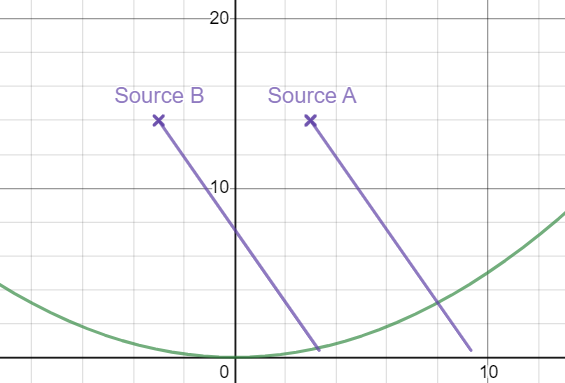
\includegraphics[scale=0.4]{source}
\end{figure}

To locate where such a ray will intersect with the parabola a little algebra is used - simply set the cartesian equations of the incident ray and the parabola equal to each other and solve for $x$, which will simply be called $p_o$ (and $q_o$ for the other incident ray).
$$ax^2=-\cot\left(\alpha\right)\left(x-r\right)+b \to x=\frac{-\cot\left(\alpha\right)+\sqrt{\cot^{2}\left(\alpha\right)+4a\left(A_{x}\cot\left(\alpha\right)+A_{y}\right)}}{2a}=p_o$$
$$ax^2=-\cot\left(\alpha\right)\left(x+r\right)+b \to x=\frac{-\cot\left(\alpha\right)+\sqrt{\cot^{2}\left(\alpha\right)+4a\left(B_{x}\cot\left(\alpha\right)+B_{y}\right)}}{2a}=q_o$$
(In using the quadratic formula, choose not to use the negative square root)

Because quadratics are differentiable (locally linear - which is why the Law of Reflection even applies), form the normal to the surface at some position $(p_o,ap_o^2)$ by parameterizing a line whose slope (found by taking the derivative, evaluating it at those x values, and converting to the slope of the normal line) is $\frac{-1}{2ap_o}$ at that position. Do the same for the location $(q_o,aq_o^2)$:
$$A:\left(t+p_{o},\frac{-1}{2ap_{o}}t+ap_{o}^{2}\right)$$
$$B:\left(t+q_{o},\frac{-1}{2aq_{o}}t+aq_{o}^{2}\right)$$

In order to proceed, we have to solve the case where the angle between the incident rays and the axis of rotation is $0\deg$. Form the incident rays which intersects at $p_o$ and $q_o$ like so:
$$A:\left(p_{o},t+ap_{o}^{2}\right)$$
$$B:\left(q_{o},t+aq_{o}^{2}\right)$$

\begin{figure}[h]
\centering{}
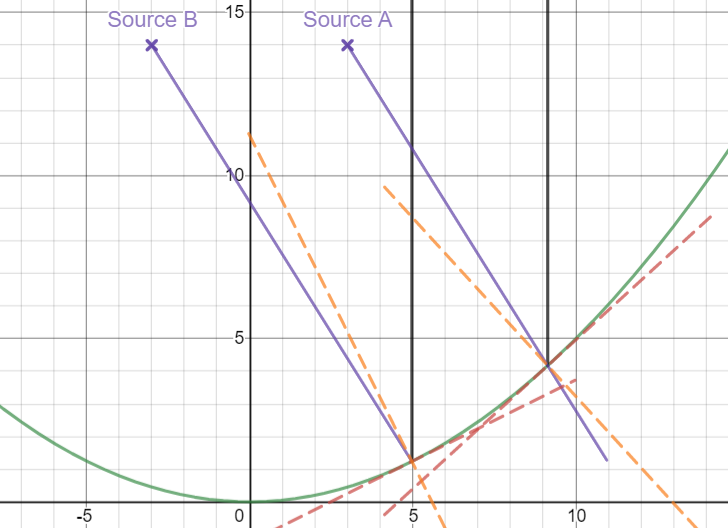
\includegraphics[scale=0.3]{pinc}
\end{figure}

To find the reflected ray, I treat the parametric definitions of the incident rays and the normal lines as vectors and find the cosine of the angle between them using the definition of the dot product. The cosine of the angle $\theta$ made between any two vectors $\vec{u}$ and $\vec{v}$ is given by:
$$\cos(\theta) = \frac{\vec{u}\cdot \vec{v}}{||\vec{u}||||\vec{v}||}$$

We symbolically form the cosine of the angle $\theta$ between the incident ray and the normal \textit{vector} (doing the $p_o$ case for demonstration) by first stripping the normal vector and the incident ray vector of its position component and shifting it back to the origin (this is to keep the math clean) by subtracting $(p_o,ap_o^2)$ from it to form a new normal: $\left(t,\frac{-1}{2ap_{o}}t\right)$ and a new incident ray: $\left(0,t\right)$. Proceed by simply using the above expression in this new context:
$$\cos(\theta)=\frac{\left(0,t\right)\cdot\left(t,\frac{-1}{2ap_{o}}t\right)}{||\left(0,t\right)||||\left(t,\frac{-1}{2ap_{o}}t\right)||} \to \cos(\theta)=\frac{\frac{-1}{2ap_{o}}}{\sqrt{1+\frac{1}{4a^2p_{o}^2}}}$$

Let some vector $\vec{\omega}$ be represented as $(X,Y)$, and suppose that it also shares the same angle with the transformed normal vector but is not equal to the transformed incident ray vector. This vector represents the direction of the reflected ray, and this method of forming it acknowledges the properties of the reflected ray as dictated by the Law of Reflection. The following expression can then be made:
$$\cos(\theta)=\frac{(X,Y)\cdot\left(t,\frac{-1}{2ap_{o}}t\right)}{||(X,Y)||||\left(t,\frac{-1}{2ap_{o}}t\right)||} \to \cos(\theta)=\frac{X+\frac{-1}{2ap_{o}}Y}{\sqrt{X^2+Y^2}\sqrt{1+\frac{1}{4a^2p_{o}^2}}}$$

Because we are sticking to principal values of $\cos(\theta)$, we do not need to worry about coterminal angles and hence we equate both expressions for $\cos(\theta)$ and solve for X and Y:
$$\frac{\frac{-1}{2ap_{o}}}{\sqrt{1+\frac{1}{4a^2p_{o}^2}}}=\frac{X+\frac{-1}{2ap_{o}}Y}{\sqrt{X^2+Y^2}\sqrt{1+\frac{1}{4a^2p_{o}^2}}} \to \sqrt{X^2+Y^2}=-2ap_oX+Y$$

An educated assumption tells us that one solution might involve $X=t$, because the reflected ray is in some aspect horizontally developed, meaning that at the very least the horizontal component can be parameterized linearly in some fashion. Plugging that in, solve for $Y$:
$$\sqrt{t^2+Y^2}=-2ap_ot+Y \to Y=ap_{o}t-\frac{t}{4ap_{o}}$$

Hence the reflected ray vector $\vec{\omega}$ can be represented as $(t,ap_{o}t-\frac{t}{4ap_{o}})$. Add back the position component we subtracted earlier from the normal and incident ray vectors to move it back to where it should be, and we get $\left(t+p_{o},ap_{o}t-\frac{t}{4ap_{o}}+ap_{o}^{2}\right)$, which if plotted together with the actual incident ray and normal line does indeed accurately reflect (intentional pun) the behavior we are trying to simulate, at least for just the $0\deg$ case. The process outlined above is no different for the incident ray at $x=q_o$.

\begin{figure}[h]
\centering{}
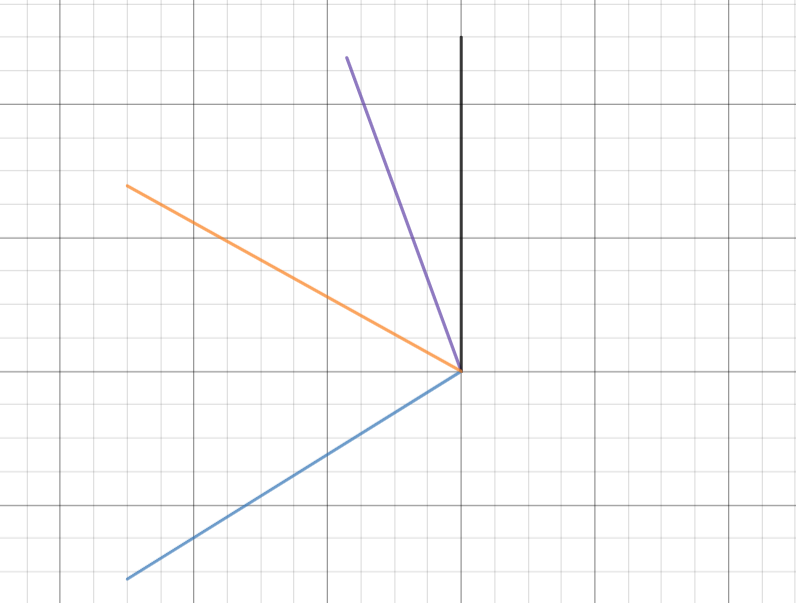
\includegraphics[scale=0.3]{vec}
\end{figure}

 As a curious side note, converting the parametric form of the reflected ray to its Cartesian form gives us $y=\left(ap_{o}-\frac{1}{4ap_{o}}\right)x+\frac{1}{4a}$, whose $y$ intercept is $\frac{1}{4a}$, which is what I learned in my precalculus class as the y value of the focus. Neat!

A key observation must be made before proceeding to work with the oblique incident ray, in superimposing both the parallel incident ray and the oblique incident ray:


\begin{figure}[h]
\centering{}
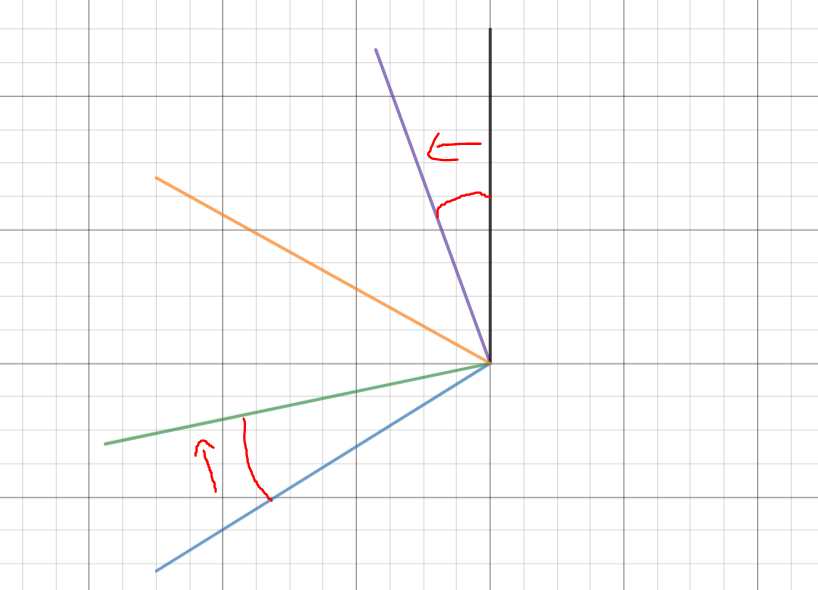
\includegraphics[scale=0.3]{vec2}
\end{figure}

The angle the incident ray makes with the axis of rotation is the same angle which the parallel incident ray is bent \textit{towards or away from} the normal line. Because the Law of Reflection holds, all we have to do to locate where the reflected ray of the oblique incident ray is to rotate the original reflected ray (from the parallel incident ray) towards the normal equally so. 

This is achieved using rotation of axes. The procedure to rotate coordinates by the angle $\theta$ (about the origin, clockwise) is given (Stewart) by the following functions:
$$X^{\prime} = X\cos(\theta)+Y\sin(\theta)$$
$$Y^{\prime} = -X\sin(\theta)+Y\cos(\theta)$$

So for something such as the reflected ray's direction (the reflected ray vector minus the position components) given by the parametric relation $\left(t,ap_{o}t-\frac{t}{4ap_{o}}\right)$, we let each component as a whole act as $X$ and $Y$ respectively and apply the transformation. This particular parameterization of the reflected ray's direction let me directly rotate them without problems, but do take care when rotating them (check via graphing). We should get the following two new reflected rays, after adding back the position components:
$$A:\left(p_{o}+t\cos\left(\alpha\right)+\left(ap_{o}t-\frac{t}{4ap_{o}}\right)\sin\left(\alpha\right),ap_{o}^{2}-t\sin\left(\alpha\right)+\left(ap_{o}t-\frac{t}{4ap_{o}}\right)\cos\left(\alpha\right)\right)$$
$$B:\left(q_{o}+t\cos\left(\alpha\right)+\left(aq_{o}t-\frac{t}{4aq_{o}}\right)\sin\left(\alpha\right),aq_{o}^{2}-t\sin\left(\alpha\right)+\left(aq_{o}t-\frac{t}{4aq_{o}}\right)\cos\left(\alpha\right)\right)$$

From here, I converted the above expressions into their Cartesian form to locate the points of intersection of reflected rays from oblique incident rays at different angles (for ease), which were the theoretical/accepted values I would compare with after doing the actual experiment.

\end{document}